\glsresetall

\section{Qiita minimizes microbiome meta-analyses from months to minutes}\label{section_qiita}

Multi-omic advances provide new insights into the function and composition of the
microbial world one study at a time. However, to properly understand relationships
between these studies we must be able to aggregate them into meta-analyses to
identify features reproducible across biospecimens and data layers, and to
generate new hypothesis. Qiita provides convenient mechanisms for these integrations
and additionally provides a web-based platform for the analysis of microbiome
studies and comparison to public studies.

Meta-analysis aggregates and analyzes data from different studies to gain insight
and statistical power by combining samples. Meta-analyses are becoming more
prominent in microbiome studies because they allow data exploration and the
generation of new hypotheses by contextualizing new data with previously published
studies. These types of studies have a rich history from Lozupone et al.’s seminal
work identifying saline vs. non-saline environments to be the dominant parameter
distinguishing microbial communities \cite{Lozupone2007} or Ley et al.’s \cite{Ley2008Worlds}
expansion placing vertebrate gut microbiome samples into the dataframe of the
environmental samples leading to the suggestion that a remarkable amount of community
specialization has occurred over evolutionary time in the vertebrate gastrointestinal tract;
to specialized fields, like the built environment \cite{Adams2015}, to the meta-analysis
discerning the biases of primers or analytical pipelines \cite{Debelius2016, Lozupone2013}.
While exciting, meta-analyses involve tremendous effort, primarily due to three common
scenarios. First, raw data are frequently not open or completely accessible (e.g., the
sequence data, the spectra, the study covariates, etc), requiring the researcher to
attempt to track down these data, often via the corresponding or first author of the
work who in turn must coordinate with the other authors. In practice, this can take
months particularly to gather all of the covariate information. In another scenario,
the authors of an existing work may make processed data available (e.g., quality
filtered sequence data, BIOM files, etc.) without details about the processing itself.
Differences in sample or data processing can lead to technical differences that outweigh
and obscure the biological differences in the data \cite{Debelius2016}. Third, while
there are common standards for sample metadata (i.e., study covariates), such as Minimum
information about any (x) sequence (MIxS) standards \cite{Yilmaz2011}, repositories under
INSDC are not required to enforce them leading to varying degrees use. Practically, this
leads to a large error prone task of integrating what a researcher believes are common
covariates between studies, and frequently this task is done manually in MS Excel; to
highlight this difficulty, a study spanning 1000 samples and 100 covariates has 100,000
cells in a spreadsheet. If you assume a human error rate of 0.1\%, it suggests you should
expect 100 errors to be present.

To address these challenges, we developed Qiita, an open-source web-based platform
focused on meta-analysis, and which allows users to go from primary data through to
analysis and publication quality figures. Qiita alleviates these issues using the
following strategies. First, we require the user to upload the rawest form of the
data possible. For example, users who leverage common sequencing platforms generally
provide either multiplexed or demultipexed gzip’d FASTQ files. Second, all processing
commands and parameters executed in Qiita are tracked allowing analyses to reason about
provenance, and to automatically reproduce an intermediate result or analysis as
necessary. For instance, this provenance information is presented to the user when
performing meta-analyses in order to allow the user to determine if the data make
sense to combine. Third, when users upload a study, the sample covariates and sample
preparation information are validated via Qiita admin’s approval against MIxS ensuring
only standards-compliant metadata are loaded into the system.

To exemplify the meta-analysis potential of Qiita we explored the combination of
3 IBD specific studies to test the replicability of subtype specific states in the
microbiome and how they relate to the healthy plane \cite{Halfvarson2017,Gevers2014},
against the HMP1 study, using both V13 and V35 16S rRNA regions \cite{Consortium2012},
and the samples of Clostridium Difficile patients that underwent a Fecal Matter
Transplant (FMT) \cite{Weingarden2015}. We trimmed all of the samples to the first
90 nucleotides (the maximum read length of the Halfvarson et al study \cite{Halfvarson2017})
and rarefied at 1,000 sequences per sample, then computed Unweighted UniFrac \cite{Lozupone2005},
and finally we performed Principal Coordinate Analysis \cite{Vazquez-Baeza2013}. From
the plot we can see the expected clustering via the body site of the sample (Figure ~\ref{qiitafig1}A).
However, when we examine only fecal samples (‘UBERON:feces’ category), we observe a clustering
pattern that can potentially be explained by the sequencing platform as previously observed
in \cite{Lozupone2013}, Figure ~\ref{qiitafig1}B. If we restrict the analysis to samples using
the same sequencing platform, we observe clustering of the different IBD subtypes as previously
reported in \cite{Gevers2014,Halfvarson2017}, Figure ~\ref{qiitafig1}C. Using this final
distance matrix, we calculated the distance from each sample to the healthy plane \cite{Halfvarson2017},
replicating the result across independent studies. Additionally, we can see that even the samples
from the C. difficile patients are further apart from the healthy plane than those from the IBD
subtypes, yet are much closer to the healthy cohort following FMT, Figure ~\ref{qiitafig1}D.

\begin{figure}[htbp]
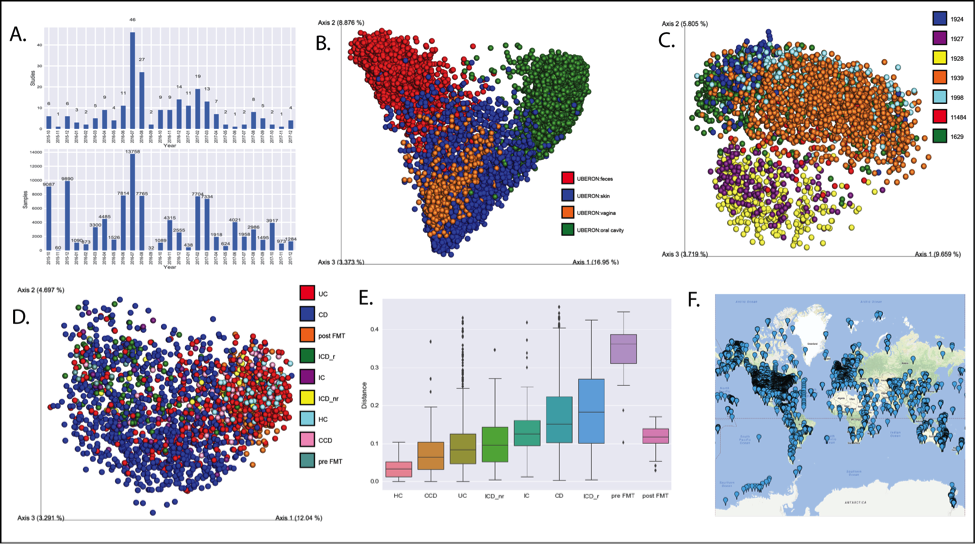
\includegraphics[width=0.75\columnwidth]{chapter_qiita_figures/Figure_1.png}
\caption[]{A. Unweighted UniFrac PCoA Meta-Analysis of three studies looking at different
IBD sub-types, one C. difficile patients that underwent an FMT, and the HMP1 and iHMP target
gene data, where we can see a nice body habitat clustering. B. Only fecal samples from the
same studies where we can see a separation due to wet-lab processing; in purple, yellow and
orange HMP1 and iHMP samples. C. After removal of those samples with different processing
we can reproduce the PCoA, which resemble previously published results on the distribution of
IBD sub-types. D. If we take the distance matrix and calculate the distance from a healthy
plane, as described in \cite{Halfvarson2017}, we can reproduce their results and even see how
the distances from the patients with a C. difficile infection have larger distances before the
FMT and shorter after. E. Geographical distribution of the samples present in the main Qiita
main deploy. F. Monthly studies and sample depositions to EBI-ENA via Qiita.}
\label{qiitafig1}
\end{figure}

Although Qiita does not require standardized metadata to perform analyses of individual datasets,
public studies available in Qiita must be MIMARKS \cite{Yilmaz2011} compliant and the metadata of
those studies has been approved by the Qiita administrators. Additionally, the Qiita administrators
can grant studies a “GOLD” tag, which represents that the study has exceptionally good metadata
and providing an example to the community. Additionally, Qiita integrates with
redbiom \footnote{\url{https://github.com/biocore/redbiom}} to rapidly search and select
studies and samples to include.

Qiita \footnote{\url{http://qiita.microbio.me}} provides storage and compute resources to
the global community, alleviating the technical burdens that are typically limiting for
biological science researchers. To date, this resource hosts over 50TB of omics data from
over 460,000 samples (of which which more than 168,000 are publicly available) originating
from studies that span the world (and outside the world), Figure  ~\ref{qiitafig1}F. Qiita
is thus an established resource for researchers who want to contextualize their data, perform
meta-analyses with already published studies, and seamlessly deposit data into EBI. Beyond these
capabilities, Qiita is positioned to democratize performing microbiome analyses by
non-bioinformaticians. Specifically, Qiita alleviates the substantial burden of maintaining
compute resources and storage, and second, provides a powerful point-and-click interface for
both sample processing and subsequent analysis, ultimately being a source of publication-quality
analyses, figures and statistics (such as those used herein). Additionally, an important
benefit of this whole process is it allows Qiita to streamline the deposition of a study
into ENA-EBI by automatically generating the necessary files, and handling the submission
when the user is ready (as has been performed now for 102,292 samples; Figure ~\ref{qiitafig1}E).

By centralizing data storage and computation, Qiita both makes meta-analyses functionality
easy for all and makes access to enormous quantities of data possible for cutting-edge resources.
A prime example of this can be Qiita workshops carried out regularly since early 2017 at UC
San Diego Center for Microbiome Innovation \footnote{\url{http://cmi-workshop.readthedocs.io/en/latest/}}.
Within 3 days we are able to educate beginner users (mostly clinicians interested in
applying microbiome to their areas of expertise): to understand and perform microbiome
analyses; metabolomics analyses; give them a forum to analyse their own data (e.g. coming
from CMI seed grants) and present their initial biological insights using publication-quality
figures, tables and statistics generated in Qiita.

\subsection{Methods}

\subsubsection{Code design and availability}

Qiita is designed using a three layer pattern: storage, logic, and interface. Each
layer will be described separately below.

The storage layer design is a combination of a PostgreSQL 9.3.17 database and a
structured filesystem. This approach allows Qiita to maintain referential integrity
within and between studies, sample metadata, the analysis pipeline(s), and the
commands executed over the different data types. However, the data volume is such
that it can encumber a relational database, so the data (e.g., sequence files,
contingency tables etc.) are stored in standard formats (e.g FASTA, FASTQ, BIOM).
The database maintains file path locations using indirection to allow files to
reside on any number of filesystems. Additionally, this layer also stores the covariates
(metadata) of each sample split in two main tables: a sample and a preparation
information. The sample information are the covariates pertinent to the sample,
while the preparation is how the sample was processed in the wet-lab and data
generation (target gene sequencing, shotgun, metabolomic, etc).

The Qiita logic layer is written in Python using Object Oriented Programming,
defining an object for each important element of the system. All data in Qiita
are represented by an “artifact” object. An artifact represents a collection of
files which reside on the filesystem, the logical types associated with each file,
and a logical type of the artifact itself. Commands can specify which type of
artifacts they accept as input and which type of artifacts they generate as output.
The type of artifacts and the commands used to analyze artifacts are defined by
Qiita plugins, which encapsulate the compute logic. Qiita defines two types of
plugins: Qiita Type Plugins and Qiita Plugins. The Qiita Type Plugins define new
artifact types, and is how data are imported into Qiita. A Qiita Type Plugin must
define only two operations: “Validate” and “Generate HTML summary”. The “Validate”
operation receives as input the set of files, and user associated types, for a new
artifact and the preparation information and determines if the set of files defines
a valid “artifact” for the given preparation. For example, in the case of a set of per
sample FASTQ files, the validator checks that each of the samples has a unique file,
and that the names of these files match those in the run\_prefix column in the preparation
information. The “Generate HTML summary” obtains the contents of an artifact and
generates an HTML file summarizing the contents of such artifact. This summary provides
a user-interpretable overview of the artifact, usually helpful enough to determine
if something went wrong with the processing of the artifact. In contrast, the Qiita
Plugin represents a collection of logically related commands (e.g., methods for
constructing distance matrices). Each command within a Qiita Plugin accepts one
or more artifacts as input, runtime parameters, and produces one or more artifacts
as output. Each command execution is logged in the Qiita relational database,
specifically, Qiita stores plugin used, the command executed within the plugin,
the artifacts provided as inputs, the parameters specified, and the artifacts generated.

The motivation for a modular plugin system is separation of concerns and encapsulation
as each plugin runs in its own discrete environment and communicates with Qiita through
an internal communication layer. This approach allows the plugins to be written in any
programming language, with plugin specific dependencies, without introducing dependency
conflicts with other plugins in the system. These environments are managed using
plugin-specific conda environments. To facilitate the development of new Qiita plugins
by external developers, we have created a Qiita client
library \footnote{\url{https://github.com/qiita-spots/qiita_client}} and two Cookiecutter
(Qiita Type Plugin \footnote{\url{https://github.com/qiita-spots/qtp-template-cookiecutter}}
\& Qiita Plugin \footnote{\url{https://github.com/qiita-spots/qp-template-cookiecutter}})
templates that set up the boilerplate code needed for setting up an initial
plugin repository and communication with Qiita.

The interface layer is a web-based interface accessible via Google Chrome,
and that is powered from the server side via Tornado 3.1.1 \footnote{\url{http://www.tornadoweb.org/}}.
The interface design and implementation has gone through multiple rounds of review,
utilizing feedback kindly provided by users attending Qiita workshops.

The source code, and comprehensive test suite, for the Qiita package can be found
in https://github.com/biocore/qiita. The source code for the officially supported
Qiita plugins can be found under the qiita-spots GitHub organization a
https://github.com/qiita-spots. All source code in the qiita repository and
qiita-spots organization are BSD-licensed.

\subsubsection{Data analysis}

One of the most important items for a successful meta-analysis is consistency
during the data processing. To achieve this consistency, Qiita limits the freedom
that users have to choose the parameters to process their raw data. The parameter
sets that are available in the system are chosen based on the recommendations
published in the literature. The parameters for demultiplexing and quality
control the 16S rRNA gene sequences are based on the assessment
performed by \cite{Bokulich2013}, while the parameters for OTU picking are based
on the recommendations provided by \cite{Navas-Molina2013}. In addition to OTU
picking, Qiita also permits sub-OTU sequence clustering with deblur \cite{Amir2017}.
In the deblur manuscript, the authors used different quality control parameters from
those outlined in \cite{Bokulich2013}.

\subsubsection{Data availability}

All data used is available via Qiita and EBI (where applicable).
The Human Microbiome Project (HMP) data is available via the HMP Data Analysis
and Coordination Center (DACC) https://hmpdacc.org/. Analytical steps for this
paper can be found in https://github.com/knightlab-analyses/qiita-paper.
